Our major goal is to provide with an efficient solution that best meet the challenges in battery charging systems using wireless power transfer.
Those challenges include:
\begin{enumerate}
\item Charging the battery as quickly as possible.
Though batteries can store large amount of charge but unfortunately there is a limit to how fast a battery can be charged and this limit gets smaller with the size (capacity) of a battery. Smaller the battery, smaller the charging current limit will be and exceeding this limit will deteriorate battery's life. To overcome this difficulty we proposed adding a super capacitor in parallel with a battery. Even though super capacitors can hold less amount of charge compared to the same size battery but they can be charged much faster \cite{IAmp}.
\item Providing long battery life with large charge to discharge ratio.
In our scenario we want to make the charging interval as small as possible which requires a need to store as much charging current as possible in this short interval and that makes the addition of super capacitor an ideal solution to overcome the battery charging limitation. During the charging interval, super capacitor can store large amount of charging current and then later use this current to charge the battery with slow pace. Which provides long battery life in terms of large charge to discharge ratio.
\item Working out efficient protocol for sharing the available charge.
\end{enumerate}

\begin{figure}[h!]
\centering
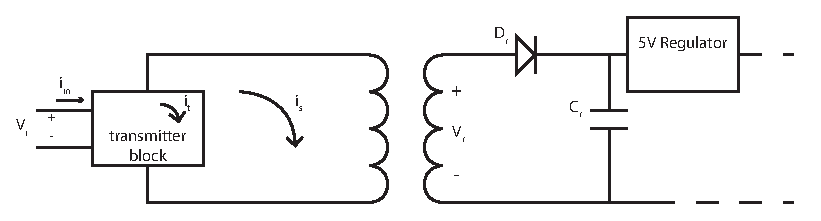
\includegraphics[width=1\textwidth]{design.pdf}
\caption{Design of the system}
\label{fig:design1}
\end{figure}

Figure \ref{fig:design1} represents the general framework of a wireless power transfer system as proposed in the assigned paper \cite{paper}. In order to propose a system design applicable to the subject of wireless power transfer we will use this framework and come up with our own parameters and design for the application. \emph{The application we will design this wireless power system for needs a regulated voltage of 5V and a maximum current of 300mA. } Based on these specifications we found a wireless power transfer set online \cite{wireless} and purchased this set as seen in figure \ref{fig:set} to build our system with. The specifications of this set are mentoined on \cite{wireless}, but will be discussed more detailed in Section \ref{sec:result}. The specifications state that the transmitter for this set requires 12V to operate and the receiver is regulated to 5V. At a distance of 1mm, more than 300mA can be coupled at 5V and the transmitted has a base current consumption of about 50mA. This set offers great possibilities as the transmitter and receiver coils are already matched on terms of frequency and a receiving IC regulates the waves into DC voltage of 5V.

\begin{figure}[h!]
\centering
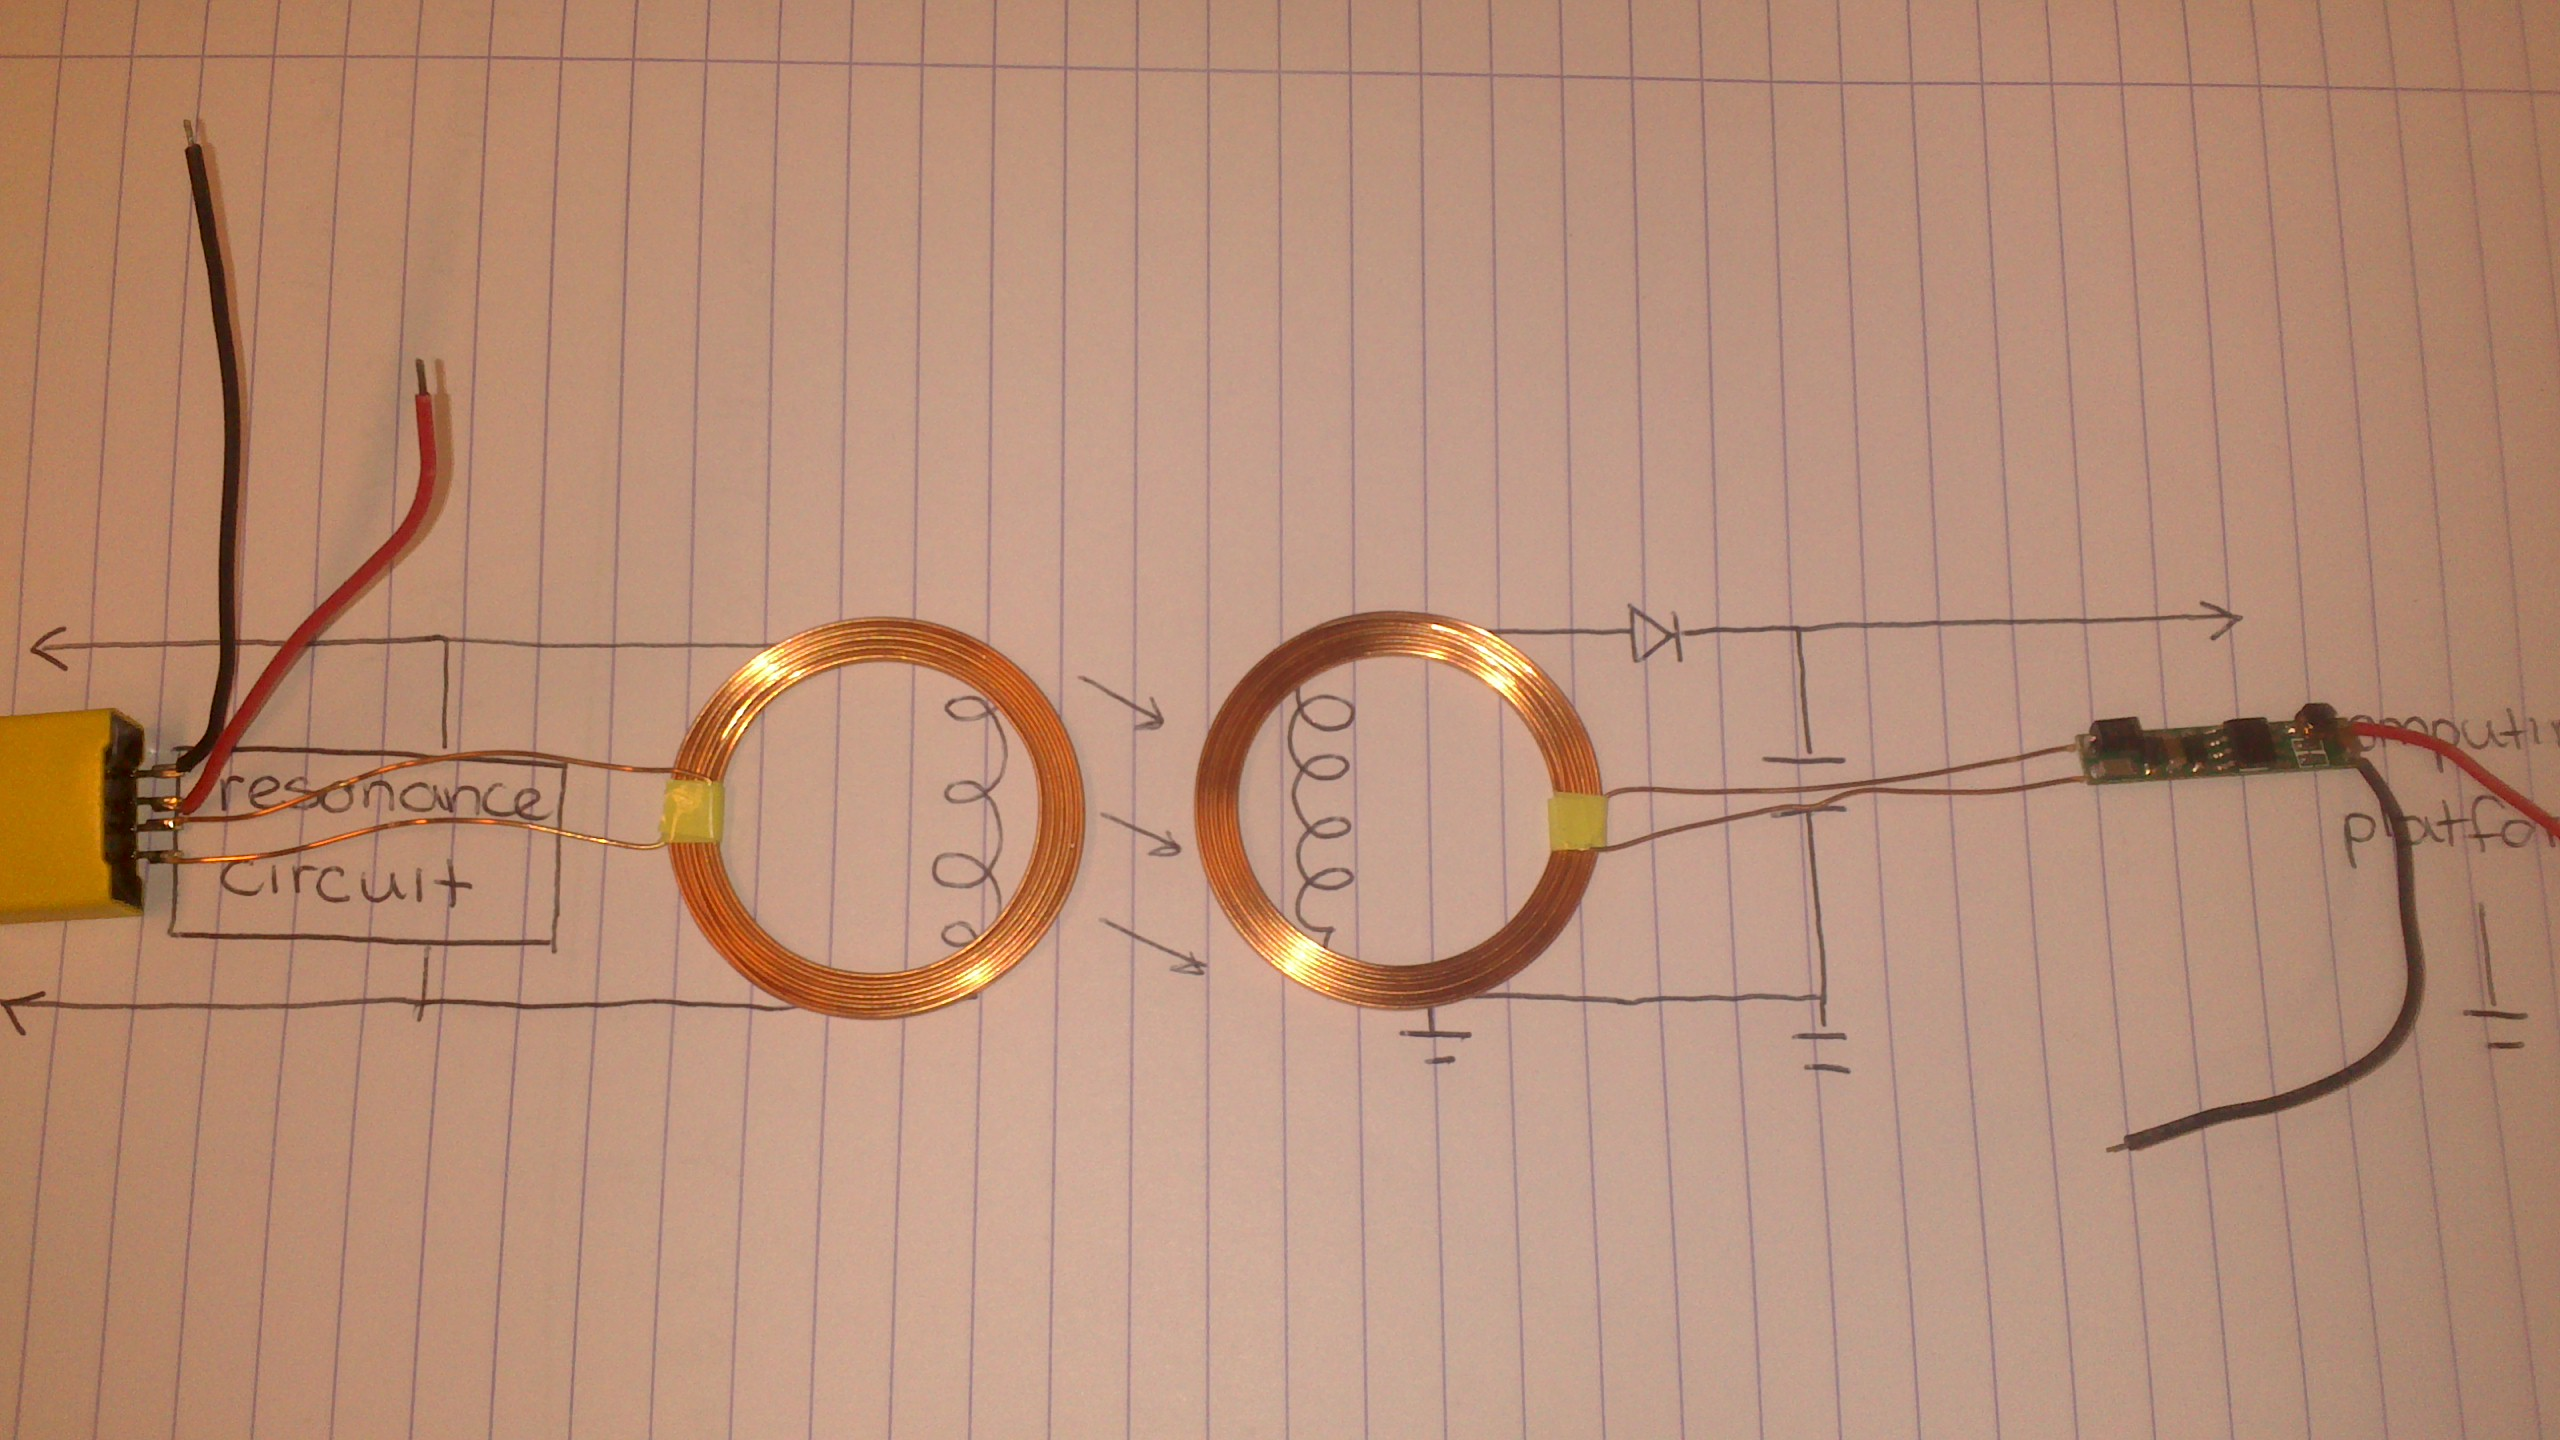
\includegraphics[width=0.7\textwidth]{wirelessset.jpg}
\caption{Engineeringshock Electronics Wireless power transfer set}
\label{fig:set}
\end{figure}